\section{Analyse des besoins fonctionnels}
\label{besoins:fonc}

\subsection{Génération de Playlist}
\label{besoins:fonc:generation}

L’objectif principal de ce projet est de générer une playlist cohérente de 
morceaux en fonction des paramètres rentrés par l’utilisateur. Cette génération 
se décompose en 2 parties distinctes.

\subsubsection{Sélection: interaction avec les données}
\label{besoins:fonc:generation:selection}

Lors de l’étape de sélection, le programme doit être capable de choisir un 
ensemble de morceaux qui correspondent aux paramètres voulus par l'utilisateur, 
tous étant optionnels. Cet ensemble est appelé la «~Pool de morceaux~». Dans le 
cas où aucune de ces options n’est fixée, la sélection des pistes doit se faire 
de manière aléatoire.

\vspace{3mm}
\noindent Les paramètres sont les suivants~:
\begin{itemize}
\item La durée de la playlist voulue, en nombre de morceaux.
\item Le nom d'un artiste/groupe.
\item Une tranche d'années.
\item Un score de popularité.
\end{itemize}

\vspace{3mm}
\noindent À ces données, on en ajoute trois basées sur le signal~:
\begin{description}
\item[Rythme~:] étant calculé d'après le tempo.
\item[Énergie~:] pouvant être calculée à partir du paramètre de «~loudness~».
\item[Humeur~:] pouvant être calculée en fonction de la tonalité du morceau 
(Note~: l’humeur n’est pas nécessairement une donnée basée sur le signal. En 
effet, le client peut très bien fournir cette information en recueillant des 
avis de personnes diverses).
\end{description}

Ces informations sont considérées comme étant exactes et fiables. Dans la base 
de données, elles sont toutes stockées dans des nombres flottants compris entre 
0 et 1. Cependant, le créateur d'une nouvelle base de données est libre 
d'imposer sa propre convention pour le calcul de ces valeurs.

\subsubsection{Ordonnancement: Similarité entre les morceaux}
\label{besoins:fonc:generation:selection:ordonnancement}

Lors de l'ordonnancement, les pistes placées dans la Pool de morceaux doivent 
être agencées tout en respectant une certaine cohérence. Un score 
de similarité est donc calculé entre les différents morceaux 
afin de repérer ceux qui sont les plus semblables.

Ce calcul doit donner un score de similarité entre deux pistes. Une playlist 
cohérente est donc une playlist dans laquelle chaque morceau possède un score 
de similarité élevé avec le morceau qui le précède et celui qui le suit.

\subsection{Visualisation de la playlist}
\label{besoins:fonc:generation:visu}

La playlist ainsi crée doit pouvoir être utilisable après avoir été générée. 
Il faut donc un moyen de la visualiser, et possiblement, de l’écouter. Le 
moyen le plus simple, mais le plus rudimentaire, est le format textuel. Ce 
format de sortie est principalement utilisé pour les tests, son utilité étant 
réduite dans les autres cas.

Un second moyen de visualiser, ou plutôt d'écouter la playlist, est d’utiliser 
un service de streaming. Celui qui a retenu notre attention est Deezer, car son 
API est en accès libre et que la construction d'une playlist est assez simple. 
Il suffit en effet d’utiliser une API javascript.
        
\subsection{Interface Utilisateur et feedback}
\label{besoins:fonc:generation:feedback}

Pour interagir avec le générateur, l’utilisateur doit passer par une interface 
(qu'elle soit graphique, ou en console) permettant de paramétrer le dit 
générateur. De plus, il est important d’envoyer un feedback des actions 
réalisées par le programme à l’utilisateur. Il faut donc utiliser un système 
nous permettant de visualiser l’avancement de la génération.

\section{Analyse des besoins non fonctionnels}
\label{besoins:nfonc}

\subsection{Performances}
\label{besoins:nfonc:perf}

Les performances lors de la génération de la playlist sont importantes, car nous
voulons éviter de frustrer les utilisateurs avec un temps d'attente trop long.

Le feedback de l’interface permet de faire patienter, mais il faut aussi 
raisonner en performance brute. Le nombre de pistes qui correspondent aux 
critères rentrés par l’utilisateur peut être énorme. Il faut donc filtrer et 
limiter le nombre de ces résultats, tout en conservant une le caractère 
aléatoire de la sélection.

Nous avons donc décidé de limiter le nombre de morceaux sur lesquels faire nos 
calculs et notre ordonnancement. Les pistes sélectionnées étant un 
sous-ensemble plus petit de tous les morceaux correspondant aux critères 
choisis, notre convention est donc de limiter ce sous-ensemble de pré-sélection 
à 10 fois la taille de playlist demandée par l’utilisateur. Ainsi, pour une 
génération de 15 morceaux, une pré-selection de 150 morceaux est effectuée, 
et la génération se fait uniquement à partir de ces morceaux. Ce système permet 
de limiter la complexité d'une génération car chaque morceau de la Pool est 
comparé à tous les autres, et ce, à chaque insertion d'une nouvelle piste dans 
la playlist. La complexité est donc de \[O(n) = n*(n*10)\], n étant la taille 
de la playlist générée.

\subsection{Modularité}
\label{besoins:nfonc:perf:mod}
    
Le projet se doit d'avoir chacune de ses parties indépendantes et remplaçables 
à souhait. Pour cela, le programme est séparé en 4 modules~:

\subsubsection{Module d'Interface Utlisateur}
\label{besoins:nfonc:perf:mod:iu}

(c.f. Section \ref{besoins:fonc:generation:feedback})

\subsubsection{Module de génération de playlist}
\label{besoins:nfonc:perf:mod:generator}

Ce module est chargé de générer la playlist en fonction d’un panel de 
descripteurs de morceaux et de paramètres. Il s'agit de la partie 
d'ordonnancement. Il est lié au module de données (c.f. Section 
\ref{besoins:nfonc:perf:mod:data}) qui se charge de la sélection des morceaux.

\subsubsection{Statégie de similarité}
\label{besoins:nfonc:perf:mod:similarity}

Ce module utilise le pattern Strategy afin de le rendre interchangeable. Cette 
classe, qui est uniquement appellée par le module de génération, contient une 
fonction qui calcule le score de similarité entre deux morceaux passés en 
paramètres.

\subsubsection{Module de données}
\label{besoins:nfonc:perf:mod:data}

Cette partie est chargée de récupérer les données pour alimenter le générateur. 
Elle peut être changée en fonction du type de données à lire (fichier(s), 
base(s) de données, etc). Nous n'avons fait qu’un seul module qui travaille 
sur une base de données SQL.

\subsubsection{Module de sortie}
\label{besoins:nfonc:perf:mod:out}

Il peut y avoir plusieurs modules de sortie s'imbriquant dans le programme, mais
il en faut au minimum un. Ce module se charge de convertir, puis de rendre à
l’utilisateur, la playlist (déjà générée par le module de génération) au 
format souhaité.

\begin{figure}[H]
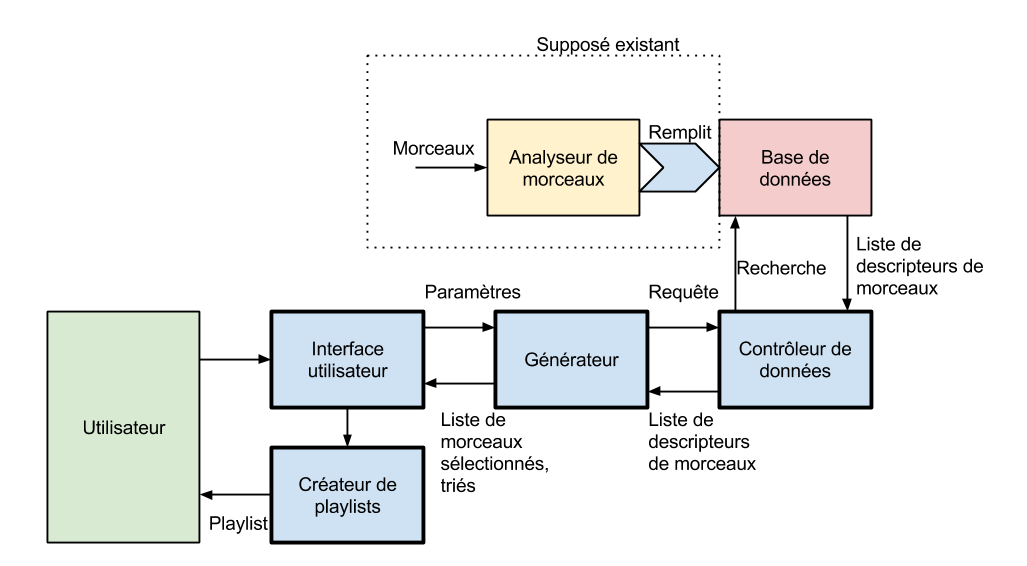
\includegraphics[width=\textwidth]{data/besoins/modules.png}
\caption{Les 4 modules indispensables au bon fonctionnement du programme et leurs
interactions.}
\end{figure}

\subsection{Ergonomie}
\label{besoins:nfonc:perf:erg}
Les interfaces doivent être utilisables par un utilisateur non-avancé et éviter 
de le perdre en étant claires et précises. Les termes employés sur cette 
interface sont donc écrits dans un vocabulaire compréhensible par tous, sans 
utiliser de mots ou d'expressions trop techniques.

\section{Contraintes}
\label{besoins:contraintes}

\subsection{Base de données}
\label{besoins:contraintes:bdd}
Nous ne disposons pas d’analyseur de morceaux, et en créer un ne fait pas partie
de notre sujet. Nous devons donc utiliser nous-même une base de données déjà
existante afin de travailler dessus. Nous avons donc choisi d’utiliser la Million
Song Dataset (http://labrosa.ee.columbia.edu/millionsong/) qui contient toutes
les informations dont nous avons besoin. Nous avons dû la convertir en base de 
données SQL afin d'améliorer le temps de récupération des données. Il nous a 
donc fallu comprendre le fonctionnement de la MSD dans le but d'écrire un 
script qui nous a permis d'en extraire les informations nécessaires pour notre 
programme et créer une base de données SQL.
    
Cette base de données pèse 500 Go, et la conversion double la place nécessaire 
pour stocker notre base de données. Bien que nous travaillons sur un 
échantillon restreint au départ, nous devons disposer d’un espace de travail 
d’au moins 1 To. Nous avons donc travaillé sur cet échantillon pour un gain de 
temps, de convertion, et de stockage.

La MSD est la seule base pouvant nous servir de test, et les informations 
qu'elle contient sont parfois très inexactes voire complétement absentes. Nous 
devons faire abstraction de ces cas particuliers, même si ils peuvent nous 
poser des problèmes dans le cadre des tests (puisque nous considérons les 
informations comme complètes et exactes).

La base de données que nous utilisons au final sera donc une conversion en base 
SQL de la Million Song Database, dont nous avons extrait uniquement les valeurs 
dont nous avons besoin.

\section{Prototypes}
\label{besoins:proto}

\subsection{Interface utilisateur graphique}
\label{besoins:proto:gui}
    
L'idée de notre interface graphique est de permettre à un utilisateur non aguérri
de faire fonctionner notre programme sans avoir de grandes connaissances en
informatique musicale. C'est pourquoi nous avons choisi de réaliser une interface
graphique simple, et au vocabulaire accessible. Par exemple, l'energie du morceau
est représentée par un curseur pouvant varier de «~léger~» à «~puissant~», sans
proposer à l'utilisateur de choisir une valeur numérique précise, ce qui ne
représenterait rien à ses yeux.
    
Les différents paramètres d'entrée sont ainsi organisés de façon à partir du plus
basique au plus complèxe, en regroupant les paramètres dits contextuels (artiste,
genre etc.) en haut, et les desripteurs audio en dessous (rythme, énergie, etc.).

Enfin nous proposons d'inclure des checkboxs afin que l'utilisateur puisse
choisir quels paramètres il veut prendre en compte, et ainsi lui laisser
la possibilité de choisir le niveau de spécification de la playlist.
    
\begin{figure}[H]
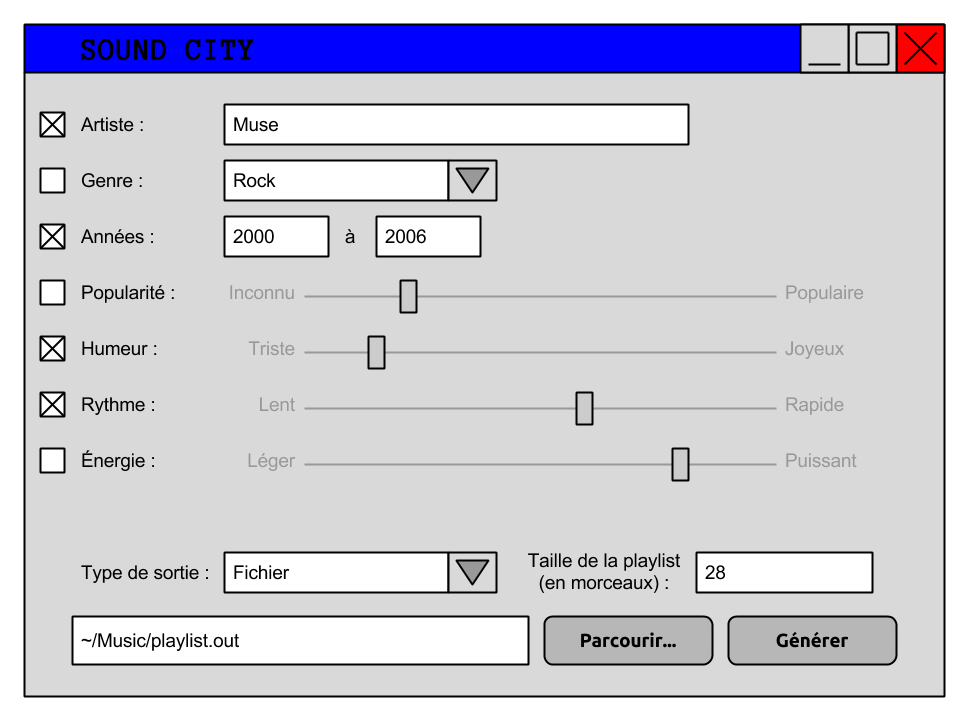
\includegraphics[width=\textwidth]{data/besoins/interface_utilisateur.png}
\caption{Prototype de l'interface utilisateur graphique.}
\end{figure}

\subsection{Interface utilisateur console}
\label{besoins:proto:console}

Cette interface possède les mêmes fonctionnalités que l'interface graphique, à 
la différence que tous les options sont placées lors de l'exécution programme :

\vspace{3mm}
\noindent Les paramètres sont les suivants~:
\begin{itemize}
\item \texttt{-y <startYear[1-3000]> <endYear[1-3000]>} : Définit un intervalle 
d'années pour les morceaux.
\item \texttt{-e <energy[0.0-1.0]>} : Impose une valeur d'énergie dans 
la playlist générée.
\item \texttt{-p <popularity[0.0-1.0]>} : Impose une valeur de popularité 
dans la playlist générée.
\item \texttt{-r <rhythm[0.0-1.0]>} : Impose un rythme dans la 
playlist générée.
\item \texttt{-m <mood[0.0-1.0]>} : Impose une humeur dans la 
playlist générée (plus la valeur est élevée, plus le morceau est joyeux).
\item \texttt{-s <size[1-100]>} : Choix de la taille de la 
playlist générée (10 par défaut).
\item \texttt{-o <fileName>} : Choix du nom du fichier de sortie.
\item \texttt{-a <artistName>} : Impose un artiste.
\end{itemize}
